\section{Implementacion}

A la hora de implementar los métodos propuestos, decidimos incluir distintas variantes de los mismos. En primer lugar, implementamos los 3 métodos como mencionamos en la sección Desarrollo. Los parametros de nuestro programa son los siguientes: \\

\begin{itemize}
  \item $originalVideo.txt $: Archivo del video original en formato de texto.
  \item $generatedVideo.txt$: Archivo donde se guarda el video interpolado en formato de texto.
  \item $method$: Método de interpolación. Puede ser 0 (Vecinos más cercanos), 1 (Lineal) o 2 (Splines)
  \item $framesToAdd$: La cantidad de frames que se desea agregar entre 2 frames. Siempre se utiliza la misma cantidad de frames agregados entre dos frames. No se implementó una variante donde se agreguen más frames en un segmento del video que en otro.
  \item $checkVSoriginal$: Puede ser $true$ o $false$. En caso de ser $true$, toma el video original y remueve $framesToAdd$ frames, dejando un frame de por medio. Por ejemplo, si tengo un video de 11 frames y $framesToAdd$ es 2, el video a procesar constaría de los frames 0, 3, 6 y 9 (el último frame es removido, y se obtendrá un video más corto que el original de no ser justo un múltiplo). Se interpolarían esos frames, y además de devolder el video interpolado, devuelve el ECM y PSNR entre los frames generados y los frames originales que fueron removidos.\\
  Si es $false$, no se remueven frames del video original.
  \item $intervalMethod$: Puede ser $block$ o $ecm$. Si es $block$, divide al video original en segmentos del tamaño del parametro que sigue. Si es $ecm$, divide al video en segmentos de acuerdo al parametro que sigue.
  \item $blockSizeOrThreshold$: Si $intervalMethod$ es $block$, el parametro debe ser un entero que indica el tamaño de bloque en que se divide el video. Cada segmento tendrá tantos frames como indique este parámetro (excpeto el último segmento de no ser un múltiplo). El tamaño debe ser mayor a 1, dado que si se dividiera en bloques de 1 frame, no hay vídeo a interpolar. Si el tamaño es la cantidad de frames del video original o mayor, no se divide el video original en segmentos y se lo toma como un solo video. \\
  Si $intervalMethod$ es $ecm$, el parametro debe ser un numero real mayor o igual a cero. Este número indica el umbral a partir del cual se debe segmentar un video. Se recorre el video original, comparando el frame $i$ con el frame $i+1$. Si el ECM es mayor al parámetro, allí se debe segmentar el vídeo. La idea original era no procesar los frames donde hubiera un cambio brusco de cámara. Sin embargo no ahondamos en esta alternativa y en la implementación interpola entre esos frames también.
\end{itemize}

Cuando sacamos frames del video original, hacemos de cuenta que el video original en realidad tiene menos frames de los que realmente tiene. En la siguiente imagen, indicamos con una X los frames que removemos, los cuales serán los que generaremos con el método propuesto.

\begin{figure}[h!]
  \centering
    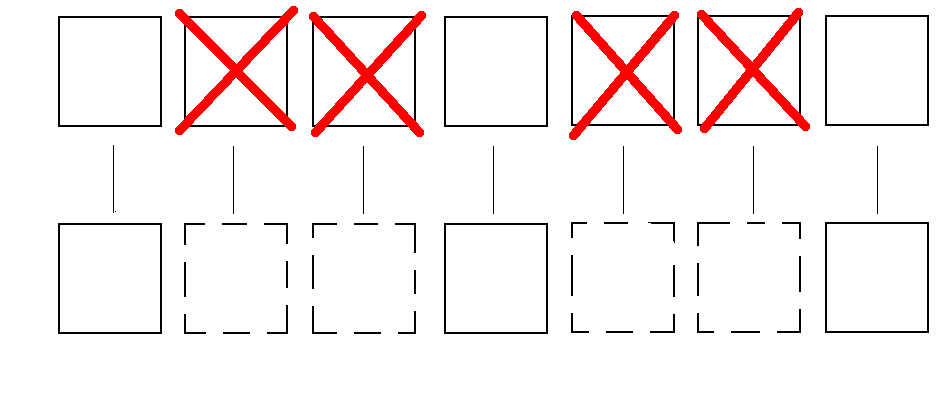
\includegraphics[scale= 0.3]{imagenes/sacandoFrames.png}
  \caption{Como se sacan frames del video original para comparar con los originales}
\end{figure}

Cuando segmentamos el video en bloques, el último frame de un bloque es el primer frame del bloque siguiente (excepto el último). Esto se debe a que, de no ser así, habria frames para los cuales no se interpolaría. Cuando se divide el método por bloques de igual tamaño, esto no parecería tener mucho sentido a menos que el video original justo tenga cambios de cámara en cada tamaño de bloque.

\begin{figure}[h!]
  \centering
    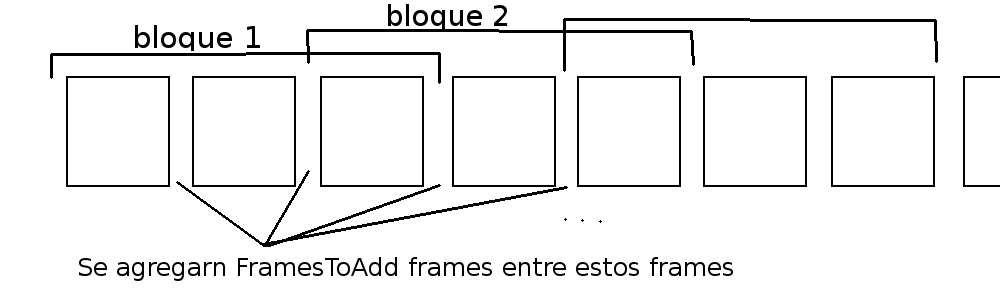
\includegraphics[scale= 0.3]{imagenes/framesToAddBloques.png}
  \caption{Como se segmenta el video en bloques}
\end{figure}


% \begin{algorithm}
% \caption{Método de la Potencia}\label{metpot}
% \begin{algorithmic}[1]

%   \Function{MetodoPotencia}{Matriz A, vector x, double c, tolerance, maxIter}%\Comment{con $A \in R^{(nxm)*(nxm)}$, $b \in R^{nxm}$}

%     \State $x = x/\lVert \mathbf{p} \rVert _{1}$
%     \While{ no se alcance la iteracion máxima}
%       \State resuelvo sistema y = A.(1-c)*x + ms
%       \State obtengo norma de y
%       \State  defino error como la norma uno de la resta entre x e y
%       \If {difieren en menos del error tolerado}
%         \State devuelvo vector y con su norma como autovalor
%       \Else
%         \State x = y
%       \EndIf
%     \EndWhile
%     \Return false
%   \EndFunction

% \end{algorithmic}
% \end{algorithm}

